\documentclass{article}
\usepackage{graphicx}


\title{Labwork 1: Gradient Descent}
\author{Phi Doan Minh Luong - 2440046}

\begin{document}

\maketitle

\setlength\parindent{0pt}

\section{Implementation}
- 2 functions f(x) and f\_(x) to find the value of f(x) and f'(x)

- First, calculate the derivative of f(x) = $x^2$ is f'(x) = 2x

- Calculate the new value of x using the gradient descent formula: x = x - L * f'(x). Loop that 10 times

- Print the value of x and f(x) each time

- Here is the result when run 10 times, with the initial value of x = 10, and the learning rate r = 0.1

\begin{center}
    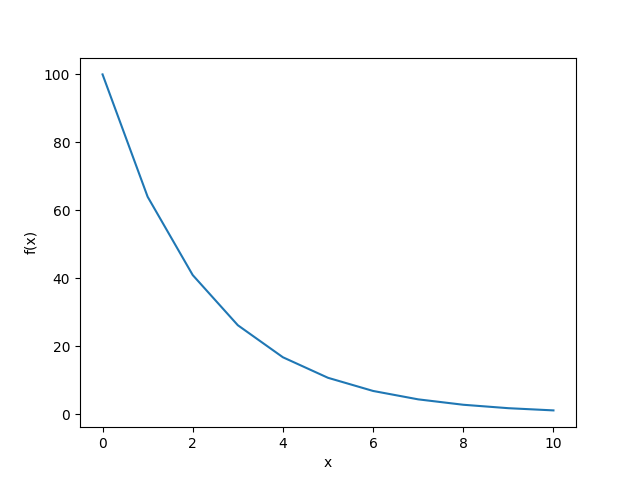
\includegraphics[width=0.5\linewidth]{image1.png}
\end{center}

\section{The effect of different learning rates}
\subsection{Learning rate is too small (0.01)}
- When the learning rate is too small, it requires many updates before reaching the minimum point

\begin{center}
    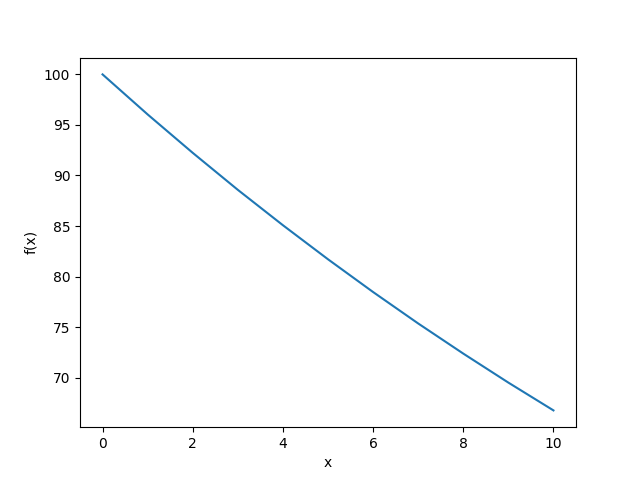
\includegraphics[width=0.5\linewidth]{image2.png}
\end{center}

- After updating 10 times, the value of f(x) is still around 70

\subsection{Learning rate is too large (0.99)}
- When the learning rate is too large, it could cause drastic updates, which lead to divergent behaviors

\begin{center}
    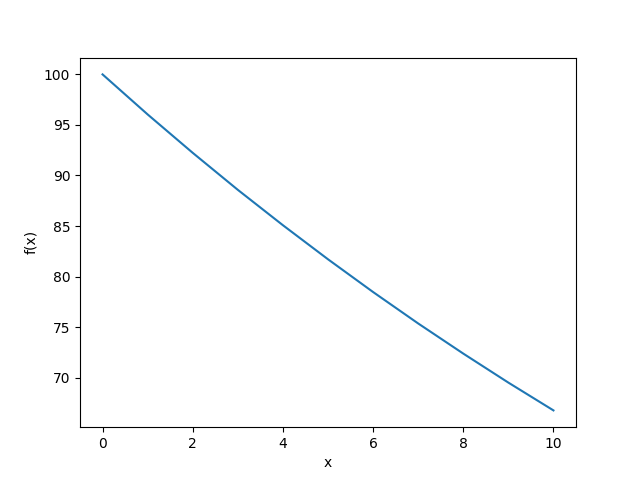
\includegraphics[width=0.5\linewidth]{image3.png}
\end{center}

- After updating 10 times, the value of f(x) is still around 70 because it overshot.

\end{document}